%{Backgrounds and systematics}
\section{Backgrounds}
While the VBF $H\rightarrow WW\rightarrow \ell\nu\ell\nu$ channel gives a fairly clear signal with $E_{\text{T}}^{\text{miss}}$, two leptons, and 2 jets, there are substantial backgrounds with similar final states. These include Drell-Yan processes (in which a $Z$ boson is formed from quark  anti-quark annihilation of the two colliding protons), top quark final states (predominantly $t\bar{t}$) and diboson events (led by SM $WW$ events), Higgs decays from the ggF production mode and finally background from mis-identified leptons, called fakes. In this section I will detail each background and describe our methods for estimating their role in our overall results. I will describe how this analysis estimates and minimizes contributions from each background process. Finally, we demonstrate purity and modelling of these backgrounds in validation and control regions. I made key contributions in this analysis in optimizing and testing control region definitions and their effects on our overall results. 
\subsection{Drell-Yan background ($Z\rightarrow \tau\tau$)}
The Drell-Yan background, alternatively called $Z\rightarrow \tau\tau$ or $Z+$jets is produced in the initial collision when two quarks produce a $Z$ boson which then decays to two leptons (in the largest background, $\tau$ leptons which then decay to electron/muons and neutrinos).  Thus there are two jets and two leptons in its final state as well as missing energy from neutrinos, all of which are indicative of signal VBF Higgs events as well. A typical Drell-Yan feynman diagram is shown in Figure \ref{fig:DrellYan}. 
\begin{figure}
\centering
  \includegraphics[width=.5\linewidth]{Pictures/FeynmanDrellYan.png}
\caption{Feynman diagram for Drell-Yan process in which two quarks produce a photon or $Z$-boson that then decays leptonically.}
\label{fig:DrellYan}
\end{figure}
The Drell-Yan background can be discriminated from our signal as well as the other backgrounds in two main ways- first in terms of the mass of the overall event aligning with the mass of the $Z$ boson. To select for Drell-Yan events we can select those which $m_{\tau\tau}$ is near the $Z$ mass peak. $m_{\tau\tau}$ is defined in the previous section and cutting on this in a 25 GeV window about the $Z$-mass peak drasticly improves our $Z+$jets purity from only 19$\%$ of total events to $\approx52\%$. 

We have also tested and trained a secondary discriminant for $Z+$jets in our analysis, a BDT trained to discriminate $Z+$jets and VBF signal events. This BDT significantly decreases overall $Z+$jets background in our signal region but we found that the subsequent decrease in statistics from using this cut leads to very similar overall results. The results from this comparison are shown in the Appendix. 

The $Z+$jets background has a very different $E_{\text{T}}^{\text{miss}}$ signature than VBF as this sample does not contain the level expected from VBF Higgs events. Thus a BDT trained to discriminate between VBF signal events and the $Z+$jets background uses a range of $E_{\text{T}}^{\text{miss}}$ variables and cutting on this trained discriminant rather directly on $E_{\text{T}}^{\text{miss}}$ provides an enhanced purity. The training and results from the BDT are described in the next subsection. Note that the following results from substantial obtimization on training inputs and techniques where the final BDT has high discrimination, no under or overtraining, and utilizes variables which are well-modelled and not highly correlated to one another.  

\subsubsection{$Z\rightarrow\tau\tau$ BDT}
A decision tree is a collection of cuts designed to classify events as signal-like or background-like. A given signal event is correctly identified if it is placed in a signal-dominated leaf and vice-cersa for background events. After the initial tree is built another tree is grown to better separate the signal and background events misidentified by the first tree. This proceeds iteratively until there is a collection of a specified number of trees, in a process known as boosting. A weighted average is taken from all these trees to form a BDT output discriminant with values ranging from -1 to 1.

The BDT is trained using $e\mu+\mu e$ events after the VBF selection and the signal regions cuts including that on $n_{jets}$, $b$-veto, OLV, CJV, $M_{jj}$ and $DY_{jj}$. In this way, the phase space in which we train the BDT is exactly the same as the one where we apply it. The training includes only the $Z\rightarrow\tau\tau$ background and the VBF signal. The MC statistics used in the training are half those available after all signal region cuts (as the other half are later used to test the training). This corresponds to $\approx$ 5,000 $Z\tau\tau$ events and $\approx$100,000 VBF events.

The TMVA BDTG interface is used to train and test the BDT. The optimal parameters were found through a scan of reasonable values and the final set is summarized in Table~\ref{tab:ZBDTparameters}.
\begin{table}[h!]
\centering
\begin{tabular}{|l|c|c|}
\hline
Parameter                                    & Value    & Range     \\
\hline
Boosting algorithm                           & Gradient & --        \\
Maximum tree depth                           &  22      & [3,10,22,30]    \\
Number of trees                              &  1000    & [200,1000,10000] \\
Minimum number of events requires per mode   &  5\%     & [5\%]\\
Number of cuts                               &  7       & [3,5,7,9]  \\
\hline
\end{tabular}
\caption{BDT parameters used for the $Z\rightarrow\tau\tau$ training.} 
\label{tab:ZBDTparameters}
\end{table}
For this BDT we aim to take advantage of the different $E_{\text{T}}^{\text{miss}}$ distributions in $Z\rightarrow\tau\tau$ backgrounds and VBF signal Monte Carlo events. Instead of a cut on $E_{\text{T}}^{\text{miss}}$, we train the BDT using multiple different $E_{\text{T}}^{\text{miss}}$ variables to maximize discrimination and then cut on the BDT output variable. Training using variables including $E_{\text{T}}^{\text{miss}}$, $\ensuremath{E_{\text{T}}^{\text{miss, track}}}$, $\ensuremath{E_{\text{T,rel}}^{\text{miss}}}$, $\ensuremath{E_{\text{T,rel}}^{\text{miss, track}}}$, $\Delta\phi_{\ell\ell,E_{\text{T}}^{\text{miss}}}$, $\Delta\phi_{\ell\ell,E_{\text{T}}^{\text{miss, track}}}$, and $\ensuremath{E_{\text{T}}^{\text{miss, significance}}}$ have been tested. The optimal analysis uses $\ensuremath{E_{\text{T}}^{\text{miss, significance}}}$, $\ensuremath{E_{\text{T}}^{\text{miss, track}}}$, $\ensuremath{E_{\text{T,rel}}^{\text{miss}}}$, and $\ensuremath{E_{\text{T,rel}}^{\text{miss, track}}}$, $\ensuremath{\Delta\phi_{\ell\ell,E_{\text{T}}^{\text{miss, track}}}}$, and $\ensuremath{\Delta\phi_{\ell\ell,E_{\text{T}}^{\text{miss}}}}$. Relative $E_{\text{T}}^{\text{miss}}$ is defined as $E_{\text{T}}^{\text{miss}} * \sin(|\Phi_{E_{\text{T}}^{\text{miss}}}\Phi_{jet}|)$, $\ensuremath{E_{\text{T}}^{\text{miss, track}}}$ is calculated from tracking detectors while $E_{\text{T}}^{\text{miss}}$ is calculated from calorimeter deposits. Finally, $\ensuremath{E_{\text{T}}^{\text{miss, significance}}}$ is a newly calibrated variable from the Jet/$E_{\text{T}}^{\text{miss}}$ group that differentiates between $E_{\text{T}}^{\text{miss}}$ from electroweak and strong interactions \cite{JETEtmiss}. While $\ensuremath{E_{\text{T}}^{\text{miss, significance}}}$ wasn't shown to increase the discrimination of the BDT due to its high correlations with $E_{\text{T}}^{\text{miss}}$, replacing this variable with $E_{\text{T}}^{\text{miss}}$ showed very similar results while reducing correlations between variables like $\ensuremath{E_{\text{T,rel}}^{\text{miss}}}$ and $\ensuremath{\Delta\phi_{\ell\ell,E_{\text{T}}^{\text{miss}}}}$. Plots shown in \ref{fig:ZjetsBDTinput} and \ref{fig:ZjetscorrSB} demonstrate the input distributions used to train the BDT and their correlations.
\begin{figure}[!htbp]
    \centering
    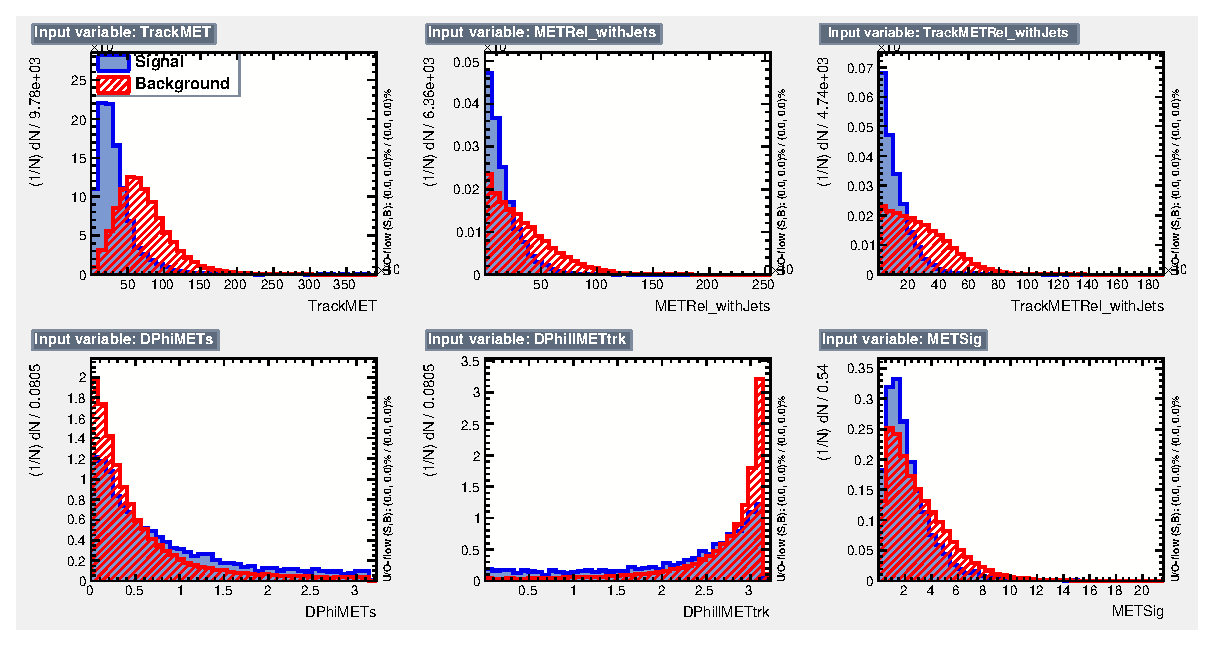
\includegraphics[width=0.85\linewidth]{Pictures/variables_id_c1.eps}
    \caption{Distributions of input variables to $Z\rightarrow\tau\tau$ BDT. Samples are unweighted and normalized to even numbers of background and signal events. Signal represents $Z\rightarrow\tau\tau$ and background VBF Higgs.}.
    \label{fig:ZjetsBDTinput}
\end{figure}
\begin{figure}[!htbp]
\centering
  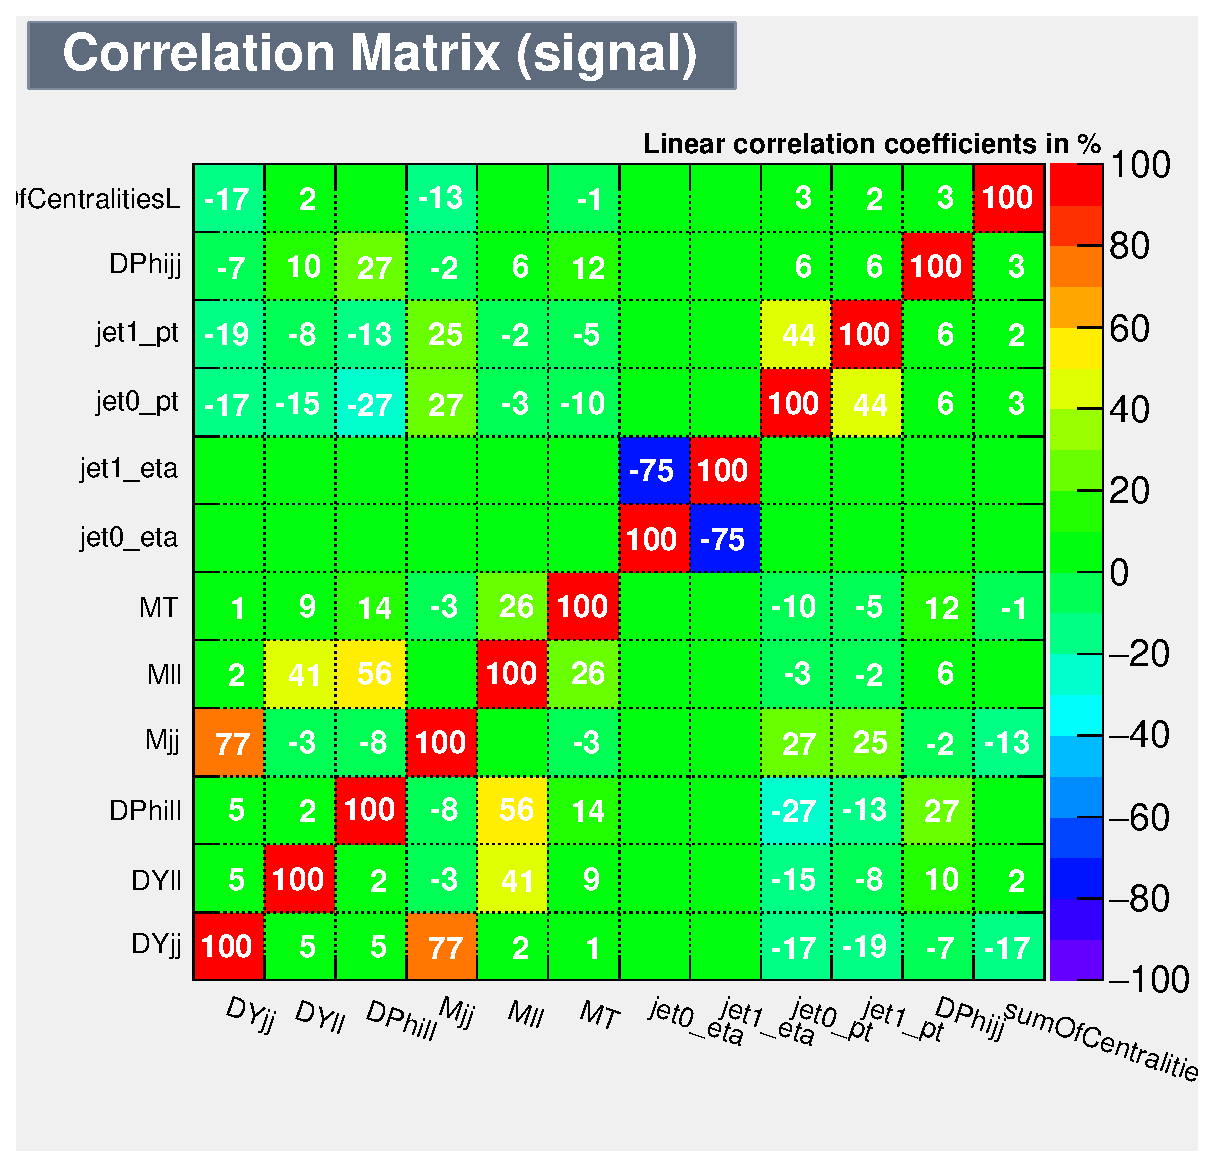
\includegraphics[width=.4\linewidth]{Pictures/CorrelationMatrixS.eps}
  \includegraphics[width=.4\linewidth]{Pictures/CorrelationMatrixB.eps}
\caption{Correlations of input variables to $Z\rightarrow\tau\tau$ BDT. Signal represents $Z\rightarrow\tau\tau$ and background VBF Higgs.}
\label{fig:ZjetscorrSB}
\end{figure}
The BDT training successfully separates $Z\rightarrow\tau\tau$ and VBF signal. In order to quantify the discrimination we use the integrated-ROC calculated through TMVA for unweighted normalized samples and find an optimal value of 0.897. Comparisons between the test and training show that the BDT is un-biased- differences between testing and training samples would imply overtraining, or the BDT using to many parameters on too few events. Visually, once can see that the testing and trainings samples are quite similar. Additionally, a Kolmogorov-Smirnov test is performed to measure if the two test and training distributions differ significantly. If the two distributions are random samples of the same parent distribution, the KS-test would give a uniformly distributed value between zero and one (or an average value of 0.5). The closer to 0.5 the KS-test, the greater likelihood the curves come from the same parent, however this calculation is heavily skewed toward lower values so any value above zero (or not very close to zero, on order $10^{-4}$) can be considered not indicative of overtraining. For signal and background we find KS-test values of 0.062 and 0.286, and so no evidence of over-training. We can visualize the BDT output variable both on un-weighted normalized samples and on samples with all event weights applied. The following plots show BDT results applied to un-weighted and weighted samples of $Z\rightarrow\tau\tau$ and VBF signal.

\begin{figure}[!htbp]
\centering
  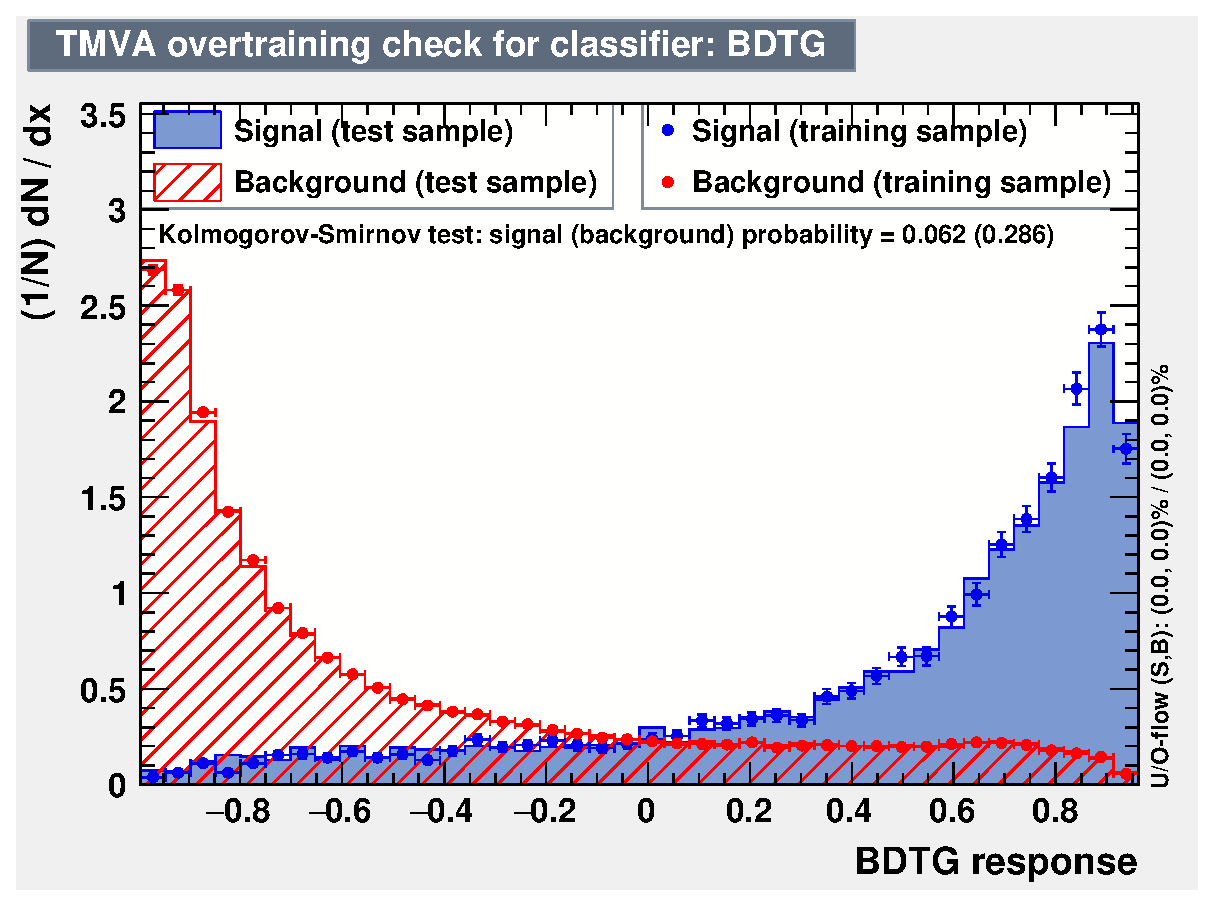
\includegraphics[width=.4\linewidth]{Pictures/overtrain_BDTG.eps}
  \includegraphics[width=.4\linewidth]{Pictures/weightedZjetsVBF.png}
\caption{Weighted, normalized samples of $Z\rightarrow\tau\tau$ (signal) and VBF (background) plotted over BDT output distribution on left, overlaid testing and training samples shown. On right, full weighted samples of $Z\rightarrow\tau\tau$ and VBF signal plotted over BDT output distributions.}
\label{fig:ZjetsBDTresult}
\end{figure}

Finally, we can test how other background samples distribute with the $Z\rightarrow\tau\tau$ BDT output variable and optimize results from cutting on this variable. The following plot \ref{fig:ZjetsBDTinterpret} shows distribution of all backgrounds as well as signal with $Z\rightarrow\tau\tau$ BDT output. We aim to increase significance while also keeping as much signal sample as possible for keep high statistics. To accomplish this we cut at a BDT output value of 0.5, in this way we eliminate $60\%$ of $Z\rightarrow\tau\tau$ background, or $\approx 450$events, and only $6\%$ of signal events. We have also tested this cut on truth samples to validate that applying this cut does not affect our fiducial phase space. 
\begin{figure}[!htbp]
\centering
\includegraphics[width=.4\linewidth]{Pictures/weightedZjetsAll.png}
\caption{Full weighted samples of all signal and background plotted over BDT output distributions}
\label{fig:ZjetsBDTintepret}
\end{figure}

\subsubsection{Drell-Yan Control Region}

The $Z+$jets control region definition is quite similar to the VBF signal region except that the $Z+$jets veto cut is inverted. Thus instead of removing events near the $Z$-mass window we select for them by applying a cut on $m_{ll}<80$ GeV,  66.2 GeV $< m_{\tau\tau}< 116.2$ GeV, and the same OLV and CJV cuts as in the VBF signal region. The $Z+$jets control region has a purity of $\approx 82\%$ and yields in this region are shown in the table below.

\begin{table}[h!]
\scalebox{0.4}{

\begin{tabular}{ r ||r  r  r | r | r  r  r | r   r }
\ensuremath{\mathcal{L}=139 fb^{-1}} & $H_{VBF}$ & $H_{ggF}$ & $H_{VH}/ttH$ & Diboson & Top & Zjets & Mis-Id & Data & Data/MC\tabularnewline
\hline
$\vert m_{\tau\tau}-m_Z\vert<$25& \ensuremath{27} & \ensuremath{84} & \ensuremath{102} & \ensuremath{2540} & \ensuremath{5635} & \ensuremath{8909} & \ensuremath{417}   & \ensuremath{16400} & \ensuremath{0.93\pm 0.01}\tabularnewline
$M_{ll}<80$ GeV & \ensuremath{26} & \ensuremath{82} & \ensuremath{84} & \ensuremath{1082} & \ensuremath{1704} & \ensuremath{8675} & \ensuremath{232}  & \ensuremath{10805} & \ensuremath{0.91\pm 0.01}\tabularnewline
CJV$<20$ GeV & \ensuremath{21} & \ensuremath{59} & \ensuremath{64} & \ensuremath{791} & \ensuremath{1151} & \ensuremath{6474} & \ensuremath{185} & \ensuremath{7931} & \ensuremath{0.91\pm 0.01}\tabularnewline
OLV & \ensuremath{16} & \ensuremath{14} & \ensuremath{21} & \ensuremath{157} & \ensuremath{292} & \ensuremath{1393} & \ensuremath{15}   & \ensuremath{1832} & \ensuremath{0.96\pm 0.03}\tabularnewline
\hline
\end{tabular}

}
\caption{Cutflow in the $Z+$jets control region.}
\label{tab:zttcr}
\end{table}

Data/MC shows decent agreement over various variable distributions as seen in the  below. In particular, modelling over variables used in the BDT are modelled well. 

\begin{figure}[!h]
\centering
  \subfloat[$m_{\tau\tau}$]{
      \includegraphics[width=0.3\textwidth]{Pictures/run2-emme-CutVBFZtautauControl_2jetinclBDT-mtt-log.pdf}
  }\hfill
  \subfloat[$p^T_{tot}$]{
      \includegraphics[width=0.3\textwidth]{Pictures/run2-emme-CutVBFZtautauControl_2jetinclBDT-PtTot-log.pdf}
  }\hfill
  \subfloat[$m_T$]{
      \includegraphics[width=0.3\textwidth]{Pictures/run2-emme-CutVBFZtautauControl_2jetinclBDT-MT-log.pdf}
  }\hfill
  \subfloat[$E_{\text{T}}^{\text{miss}}$]{
      \includegraphics[width=0.3\textwidth]{Pictures/run2-emme-CutVBFZtautauControl_2jetinclBDT-MET-log.pdf}
  }\hfill
  \subfloat[$\ensuremath{E_{\text{T,rel}}^{\text{miss}}}$]{
      \includegraphics[width=0.3\textwidth]{Pictures/run2-emme-CutVBFZtautauControl_2jetinclBDT-METRel-log.pdf}
  }\hfill
  \subfloat[$\ensuremath{E_{\text{T}}^{\text{miss, significance}}}$]{
      \includegraphics[width=0.3\textwidth]{Pictures/run2-emme-CutVBFZtautauControl_2jetinclBDT-METSig-log.pdf}
  }\hfill
  \subfloat[$\ensuremath{E_{\text{T}}^{\text{miss, track}}}$]{
      \includegraphics[width=0.3\textwidth]{Pictures/run2-emme-CutVBFZtautauControl_2jetinclBDT-TrackMET-log.pdf}
  }\hfill
  \subfloat[$\ensuremath{E_{\text{T,rel}}^{\text{miss, track}}}$]{
      \includegraphics[width=0.3\textwidth]{Pictures/run2-emme-CutVBFZtautauControl_2jetinclBDT-TrackMETRel-log.pdf}
  }\hfill
  \subfloat[$\ensuremath{\Delta\phi_{\ell\ell,E_{\text{T}}^{\text{miss, track}}}}$]{
      \includegraphics[width=0.3\textwidth]{Pictures/run2-emme-CutVBFZtautauControl_2jetinclBDT-DPhillMETtrk-log.pdf}
  }%\hfill 
{\caption{Distributions of $m_{\tau\tau}$, $p^T_{tot}$, $m_T$, in $\ensuremath{E_{\text{T,rel}}^{\text{miss}}}$, $\ensuremath{E_{\text{T}}^{\text{miss, significance}}}$, $\ensuremath{E_{\text{T}}^{\text{miss, track}}}$, $\ensuremath{E_{\text{T,rel}}^{\text{miss, track}}}$, $\ensuremath{\Delta\phi_{\ell\ell,E_{\text{T}}^{\text{miss, track}}}}$ in the $Z+$jets control region.
\label{fig:DYCR3}}}
\end{figure}
The BDT that discriminates VBF signal and $Z+$jets is applied in the $Z+$jets control region to maintain orthogonality. This further increases purity in the control region. This distribution is shown in the following plot. 
\begin{figure}[!htbp]
\centering
\includegraphics[width=.6\linewidth]{Pictures/run2-emme-CutVBFZtautauControl_2jetinclBDT-BDT_Zjets-log.pdf}
\caption{Full weighted samples of all signal and background plotted over BDT output distributions in $Z+$jets control region after cut on $Z+$jets BDT}
\label{fig:ZjetsBDTCR}
\end{figure}
Normalization factors (NF) are derived in the $Z+$jets control region to correct for Data/MC mis-modelling. These factors are applied to the $Z+$jets sample in the signal region. The NF factors are $1.03 \pm 0.05$. 

\subsection{Top background}
The top background consists of two main components, $Wt$ and $t\bar{t}$ events where the $W$ decays leptonically and the top quarks decay to jets (notably $b$-jets). The top background is dominated by $t\bar{t}$ and is the largest background in our signal region, composing about $60\%$ of the total background. Though top backgrounds are numerous, discrimination between top and signal Higgs events is possible through training a BDT on variables that have very different discributions between these two types of events like $m_{\ell\ell}$ and $\Delta Y_{jj}$. This BDT discriminates between signal and top background quite well and so the top background is defined in the signal region and separated using this variable. The final BDT used in the final statistical fit is discused in the following chapter. We define a top validation region to test top Monte Carlo modelling as well as to calculate a normalization factor that is used to correct top mis-modelling in the signal region. The top validation region is described similarly to the signal region with one major difference, a $b$- tag applied in the signal region requiring all events with a $b$-jet to be removed is (almost) reversed. Instead we require exactly one $b$-tagged jet. We require exactly one in order to define the validation region as similarly to the signal region as possible while increasing top purity. The results is a highly pure top validation region where the flavor composition of the tagged jets is close to the signal region. Purity of the top control region is $\approx 97\%$ and yields in this region are shown in the table below.

\begin{table}[h!]
\scalebox{0.4}{
%%% created on Thu Jun 11 11:37:17 2020 from TQSampleFolder 'samples' with TQLibrary UNKNOWN compiled with GCC 8.3.0 against ROOT 6.16/00
\providecommand{\xmark}{{\sffamily \bfseries X}}
\providecommand\rotatecell[2]{\rotatebox[origin=c]{#1}{#2}}
\begin{tabular}{ r ||r  r  r | r | r  r  r | r   r }
\ensuremath{\mathcal{L}=139 fb^{-1}} & $H_{VBF}$ & $H_{ggF}$ & $H_{VH}/ttH$ & Diboson & Top & Zjets & Mis-Id & Data & Data/MC\tabularnewline
\hline
$n_{b-jets} = 1$ & \ensuremath{39.79\pm 0.19} & \ensuremath{162.38\pm 1.34} & \ensuremath{89.41\pm 0.57} & \ensuremath{3922.22\pm 31.68} & \ensuremath{349820.12\pm 128.80} & \ensuremath{3683.96\pm 34.18} & \ensuremath{4601.97\pm 97.54} & \ensuremath{359758} & \ensuremath{0.99\pm 0.00}\tabularnewline
$Z\to\tau\tau$ veto & \ensuremath{18.05\pm 0.13} & \ensuremath{22.85\pm 0.50} & \ensuremath{5.66\pm 0.13} & \ensuremath{245.35\pm 12.82} & \ensuremath{30023.80\pm 38.13} & \ensuremath{180.86\pm 8.66} & \ensuremath{280.21\pm 28.51}  & \ensuremath{30709} & \ensuremath{1.00\pm 0.01}\tabularnewline
CJV $<20$ GeV & \ensuremath{29.69\pm 0.17} & \ensuremath{106.25\pm 1.08} & \ensuremath{62.42\pm 0.47} & \ensuremath{2518.28\pm 26.99} & \ensuremath{238659.28\pm 107.33} & \ensuremath{2487.15\pm 30.44} & \ensuremath{2941.00\pm 80.13} & \ensuremath{244811} & \ensuremath{0.99\pm 0.00}\tabularnewline
OLV & \ensuremath{20.85\pm 0.14} & \ensuremath{25.71\pm 0.53} & \ensuremath{13.85\pm 0.20} & \ensuremath{411.01\pm 13.96} & \ensuremath{46267.04\pm 47.47} & \ensuremath{499.81\pm 12.91} & \ensuremath{415.70\pm 35.23}\  & \ensuremath{47182} & \ensuremath{0.99\pm 0.00}\tabularnewline
$Z\to\tau\tau$ veto & \ensuremath{18.05\pm 0.13} & \ensuremath{22.85\pm 0.50} & \ensuremath{5.66\pm 0.13} & \ensuremath{245.35\pm 12.82} & \ensuremath{30023.80\pm 38.13} & \ensuremath{180.86\pm 8.66} & \ensuremath{280.21\pm 28.51} & \ensuremath{30709} & \ensuremath{1.00\pm 0.01}\tabularnewline
\hline
\end{tabular}

}
\caption{Cutflow in the top control region.}
\label{tab:topcr}
\end{table}

Data/MC in the top validation region shows good agreement over various variable distributions as seen in the  below. 

\begin{figure}[!h]
\centering
  \subfloat[$m_{\ell\ell}$]{
      \includegraphics[width=0.3\textwidth]{Pictures/run2-emme-CutVBFTopControl_2jetinclZttVeto-Mll-log.pdf}
  }\hfill
  \subfloat[$\Delta Y_{\ell\ell}$]{
      \includegraphics[width=0.3\textwidth]{Pictures/run2-emme-CutVBFTopControl_2jetinclZttVeto-DYll-log.pdf}
  }\hfill 
  \subfloat[$\Delta Y_{jj}$]{
      \includegraphics[width=0.3\textwidth]{Pictures/run2-emme-CutVBFTopControl_2jetinclZttVeto-DYjj-log.pdf}
  }\hfill
  \subfloat[$m_{jj}$]{
      \includegraphics[width=0.3\textwidth]{Pictures/run2-emme-CutVBFTopControl_2jetinclZttVeto-Mjj-log.pdf}
  }\hfill
  \subfloat[$\Delta\Phi_{jj}$]{
      \includegraphics[width=0.3\textwidth]{Pictures/run2-emme-CutVBFTopControl_2jetinclZttVeto-DPhijj-log.pdf}
  }\hfill
  \subfloat[$p^T_{tot}$]{
      \includegraphics[width=0.3\textwidth]{Pictures/run2-emme-CutVBFTopControl_2jetinclZttVeto-PtTot-log.pdf}
  }\hfill
  \subfloat[$m_T$]{
      \includegraphics[width=0.3\textwidth]{Pictures/run2-emme-CutVBFTopControl_2jetinclZttVeto-MT-log.pdf}
  }\hfill
  \subfloat[$\ensuremath{E_{\text{T,rel}}^{\text{miss}}}$]{
      \includegraphics[width=0.3\textwidth]{Pictures/run2-emme-CutVBFTopControl_2jetinclZttVeto-MET-log.pdf}
  }%\hfill 
{\caption{Distributions of $m_{\ell\ell}$, $\Delta Y_{\ell\ell}$, $\Delta Y_{jj}$, $m_{jj}$, $\Delta\Phi_{jj}$, $p^T_{tot}$, $m_T$, and $\ensuremath{E_{\text{T,rel}}^{\text{miss}}}$ in the top validation region.
\label{fig:TopCR3}}}
\end{figure}
The BDT to discriminate top background from VBF signal events is trained and applied in the signal region and so described in the next chapter, but its distribution in the top validation region is shown below. This BDT discriminates both WW and top (combined) against the VBF signal as they have similar kinematic distributions and are treated together in the final simultaneous fit. 

\begin{figure}[!htbp]
\centering
\includegraphics[width=.6\linewidth]{Pictures/run2-emme-CutVBFTopControl_2jetinclZttVeto-BDT_VBF-log.pdf}
\caption{Full weighted samples of all signal and background plotted over Top + $WW$ vs. VBF BDT output distributions in top validation region}
\label{fig:VBFTopWWBDTVR}
\end{figure}

A designated BDT discriminates between top and WW backgrounds and is described further in the WW background section (next). However, this distribution in the top validation region with all weighted samples is shown below. 

\begin{figure}[!htbp]
\centering
\includegraphics[width=.6\linewidth]{Pictures/run2-emme-CutVBFTopControl_2jetinclZttVeto-BDT_TopWW-log.pdf}
\caption{Full weighted samples of all signal and background plotted over Top vs. $WW$ BDT output distributions in top validation region}
\label{fig:TopWWBDTVR}
\end{figure}

Normalization factors (NF) are derived in the top validation region to correct for data/MC mis-modelling. These factors are applied to the top sample in the signal region. The NF factors are $0.99\pm0.01$. 

\subsection{Diboson background}

The $WW$ background consists primarily of QCD $WW$+jets events (highly dominating electroweak vertices). This background is estimated along with the top background using a joint parameter due to their similarities in signature as well as the difficulty in defining a pure $WW$ control region (without top contamination). A $WW$ validation region is defined to demonstrate $WW$ MC modelling in a targeted $WW$ region.  The $WW$ validation region is defined with at least 2 jets, a $b$-veto $N_{b-jet}<1$ and a central-jet-veto of below $20$GeV as in the signal region. Two additional cuts differ from the signal region - $m_T>130$GeV and $m_{T2}>160$GeV where $m_{T2}$ is defined as
\begin{equation}
m_{T2}=min_{p_T^1+p_T^2=p_T}(max(m_T^2(p_T^1,p_T^a),m_T^2(p_T^2,p_T^b)))
\end{equation}
This represents a lower bound on the parent particle's mass, so using a large $m_{T2}$ cut eliminates contamination from many $t\bar{t}$ decays which have an upper limit near the top mass. The purity of the region is $\approx 37\%$ and the cutflow for this region is shown below.

\begin{table}[h!]
\scalebox{0.4}{
%%% created on Thu Jun 11 11:37:17 2020 from TQSampleFolder 'samples' with TQLibrary UNKNOWN compiled with GCC 8.3.0 against ROOT 6.16/00
\providecommand{\xmark}{{\sffamily \bfseries X}}
\providecommand\rotatecell[2]{\rotatebox[origin=c]{#1}{#2}}
\begin{tabular}{ r ||r  r  r | r | r  r  r | r   r }
\ensuremath{\mathcal{L}=139 fb^{-1}} & $H_{VBF}$ & $H_{ggF}$ & $H_{VH}/ttH$ & Diboson & Top & Zjets & Mis-Id & Data & Data/MC\tabularnewline
\hline
b-veto & \ensuremath{324} & \ensuremath{1110} & \ensuremath{438} & \ensuremath{25107} & \ensuremath{63788} & \ensuremath{22151} & \ensuremath{3794} & \ensuremath{109677} & \ensuremath{0.94\pm 0.00}\tabularnewline
$M_{T}>$130 GeV & \ensuremath{32} & \ensuremath{155} & \ensuremath{60} & \ensuremath{18021} & \ensuremath{50088} & \ensuremath{872} & \ensuremath{1784}  & \ensuremath{68255} & \ensuremath{0.96\pm 0.00}\tabularnewline
$M_{T2}>$160 GeV & \ensuremath{19} & \ensuremath{62} & \ensuremath{17} & \ensuremath{7272} & \ensuremath{11553} & \ensuremath{302} & \ensuremath{516} & \ensuremath{18672} & \ensuremath{0.95\pm 0.01}\tabularnewline
CJV (20GeV) & \ensuremath{14} & \ensuremath{41} & \ensuremath{11} & \ensuremath{4861} & \ensuremath{6416} & \ensuremath{185} & \ensuremath{328}  & \ensuremath{11245} & \ensuremath{0.95\pm 0.01}\tabularnewline
\hline
\end{tabular}

}
\caption{Cutflow in the $WW$ validation region.}
\label{tab:wwvr}
\end{table}

Data/MC shows good agreement over various variable distributions as seen in the  below. 
\begin{figure}[!h]
\centering
  \subfloat[$m_{\ell\ell}$]{
      \includegraphics[width=0.3\textwidth]{Pictures/run2-emme-CutVBFWWControl_CJV20-Mll-log.pdf}
  }\hfill
  \subfloat[$\Delta Y_{\ell\ell}$]{
      \includegraphics[width=0.3\textwidth]{Pictures/run2-emme-CutVBFWWControl_CJV20-DYll-log.pdf}
  }\hfill
  \subfloat[$\Delta Y_{jj}$]{
      \includegraphics[width=0.3\textwidth]{Pictures/run2-emme-CutVBFWWControl_CJV20-DYjj-log.pdf}
  }\hfill
  \subfloat[$m_{jj}$]{
      \includegraphics[width=0.3\textwidth]{Pictures/run2-emme-CutVBFWWControl_CJV20-Mjj-log.pdf}
  }\hfill
  \subfloat[$\Delta\Phi_{jj}$]{
      \includegraphics[width=0.3\textwidth]{Pictures/run2-emme-CutVBFWWControl_CJV20-DPhijj-log.pdf}
  }\hfill
  \subfloat[$p^T_{tot}$]{
      \includegraphics[width=0.3\textwidth]{Pictures/run2-emme-CutVBFWWControl_CJV20-PtTot-log.pdf}
  }\hfill
  \subfloat[$m_T$]{
      \includegraphics[width=0.3\textwidth]{Pictures/run2-emme-CutVBFWWControl_CJV20-MT-log.pdf}
  }\hfill
  \subfloat[$\ensuremath{E_{\text{T,rel}}^{\text{miss}}}$]{
      \includegraphics[width=0.3\textwidth]{Pictures/run2-emme-CutVBFWWControl_CJV20-MET-log.pdf}
  }%\hfill 
{\caption{Distributions of $m_{\ell\ell}$, $\Delta Y_{\ell\ell}$, $\Delta Y_{jj}$, $m_{jj}$, $\Delta\Phi_{jj}$, $p^T_{tot}$, $m_T$, and $\ensuremath{E_{\text{T,rel}}^{\text{miss}}}$ in the $WW$ validation region.
\label{fig:WWCR3}}}
\end{figure}

The BDT to discriminate $WW$ background from VBF signal events is trained and applied in the signal region and so described in the next chapter, but its distribution in the $WW$ validation region is shown below. This BDT discriminates both WW and top (combined) against the VBF signal as they have similar kinematic distributions and are treated together in the final simultaneous fit.

\begin{figure}[!htbp]
\centering
\includegraphics[width=.6\linewidth]{Pictures/run2-emme-CutVBFWWControl_CJV20-BDT_VBF-log.pdf}
\caption{Full weighted samples of all signal and background plotted over Top + $WW$ vs. VBF BDT output distributions in $WW$ validation region}
\label{fig:VBFWWTopBDTVR}
\end{figure}

A designated BDT discriminates between top and WW backgrounds in the signal region...\textcolor{red}{need to put in BDT training information, Sagar?}

\begin{figure}[!htbp]
\centering
\includegraphics[width=.6\linewidth]{Pictures/run2-emme-CutVBFWWControl_CJV20-BDT_TopWW-log.pdf}
\caption{Full weighted samples of all signal and background plotted over BDT output distributions in WW validation region}
\label{fig:TopWWBDTVR}
\end{figure}

\subsection{ggF background}
The Higgs production via gluon--gluon fusion is estimated simultaneously from three control regions and the signal region. The control regions are chosen such as the both to minimize both the statistical and the modelling uncertainties, in particular these originating from the modelling of higher oder QCD corrections. In particular, the regions inspired from a subdivision based on the jet multiplicity. The first region, CRGGF1, is build based from the preselection and selecting events with $0$ and $1$ jet. The second and third regions, are constructed starting from the preselection and inverting the VBF selection cuts, such as to mininmize the extrapolation uncertainties to the signal region. In particular, the definitions are the following: 
\begin{itemize} 
\item {\textbf GGF-CR1} Preselection criteria and $N_{ \text{j}}<2$. 
\item {\textbf GGF-CR2} Preselection criteria and $\text{CJV} > 1$ and $\text{OLV} > 1$
\item {\textbf GGF-CR3} Preselection criteria and $\text{CJV}<1$ and $\text{OLV}>1$ or $\text{CJV}>1$ and $\text{OLV}<1$ 
\end{itemize} 
\noindent from this the expectation in the signal region is build from the following ratio, inspired from the  ABCD method, 
\begin{equation}
	\mu_{{\text GGF-SR}} = \frac{\mu^{{\text GGF-CR}}_{1} \cdot\mu^{{\text GGF-CR}}_{2}}{ \mu^{{\text GGF-CR}}_{3}}.
\end{equation}
\noindent where $\mu_{\text{GGF-X}}$ denotes the yield modifier in each region GGF-X notextalised to the expectation from simulation. The final event yield in the signal region $\mu_{{\text GGF-SR}}$ is detetextined in the simultaneous fit as described in Sec~\ref{sec:fit}. In each $gg$F category the ggF yield is extracted from simulation-extracted template fits based on dedicated discriminants. 

For each category, a dedicated multivariate discriminant is trained and applied to discriminate between $gg$F and the backgrounds. Each of these trainings is discussed next. 

\subsubsection{Discriminant in the GGF-CR1}
The multivariate discriminate used for the GGF CR1 is a boosted decision tree (BDT) trained using $e\mu+\mu e$ events that pass all ggF CR1 cuts. The training includes ggF events trained against VBF signal and all backgrounds. The MC statistics used in the training are half those available after the ggF CR1 cuts (as the other half are later used to test the training). This corresponds to $\approx$ 3,200 ggF events and $\approx$480,000 other signal and background events.

The TMVA BDTG interface is used to train and test the BDT. The optimal parameters were found through a scan of reasonable values and the final set is summarized in Table~\ref{tab:ggFCR1BDTparameters}.
\begin{table}[h!]
\centering
\begin{tabular}{|l|c|c|}
\hline
Parameter                                    & Value     \\
\hline
Boosting algorithm                           & Gradient \\
Maximum tree depth                           &  10      \\
Number of trees                              &  100    \\
Minimum number of events requires per mode   &  5\%     \\ 
Number of cuts                               &  7       \\
\hline
\end{tabular}
\caption{BDT parameters used for the ggF CR1 training.}
\label{tab:ggFCR1BDTparameters}
\end{table}
For this BDT various distributions are used to take advantage of differences in distributions between ggF events and other sample types. These variables include $\Delta Y_{\ell\ell}$, $\Delta \Phi_{\ell\ell}$,$m_{\ell\ell}$,$m_T$,$p^T_{tot}$, lep $p^T_{\text{lead}}$, lep $p^T_{\text{sublead}}$, jet $p^T_{\text{lead}}$, jet $p^T_{\text{sublead}}$, $\Delta \Phi_{jj}$, and $\ensuremath{E_{\text{T,rel}}^{\text{miss}}}$. Distributions for these variables in the ggF CR1 region where the BDT is trained are shown below demonstrating data/MC modelling for each.
\begin{figure}[!h]
  \subfloat[$\Delta Y_{\ell\ell}$]{
      \includegraphics[width=0.3\textwidth]{Pictures/run2-emme-CutVBFggFCR1-DYll-log.pdf}
  }\hfill
  \subfloat[$\Delta \Phi_{\ell\ell}$]{
      \includegraphics[width=0.3\textwidth]{Pictures/run2-emme-CutVBFggFCR1-DPhill-log.pdf}
  }\hfill
  \subfloat[$m_{\ell\ell}$]{
      \includegraphics[width=0.3\textwidth]{Pictures/run2-emme-CutVBFggFCR1-Mll-log.pdf}
  }\hfill
  \subfloat[$m_T$]{
      \includegraphics[width=0.3\textwidth]{Pictures/run2-emme-CutVBFggFCR1-MT-log.pdf}
  }\hfill
  \subfloat[$p^T_{tot}$]{
      \includegraphics[width=0.3\textwidth]{Pictures/run2-emme-CutVBFggFCR1-PtTot-log.pdf}
  }\hfill
  \subfloat[lep $p^T_{\text{lead}}$]{
      \includegraphics[width=0.3\textwidth]{Pictures/run2-emme-CutVBFggFCR1-leadLepPt-log.pdf}
  }\hfill
  \subfloat[jet $p^T_{\text{lead}}$]{
      \includegraphics[width=0.3\textwidth]{Pictures/run2-emme-CutVBFggFCR1-leadJetPt-log.pdf}
  }\hfill
  \subfloat[lep $p^T_{\text{sublead}}$]{
      \includegraphics[width=0.3\textwidth]{Pictures/run2-emme-CutVBFggFCR1-subleadLepPt-log.pdf}
  }\hfill
  \subfloat[jet $p^T_{\text{sublead}}$]{
      \includegraphics[width=0.3\textwidth]{Pictures/run2-emme-CutVBFggFCR1-subleadJetPt-log.pdf}
  }\hfill
  \subfloat[$\Delta \Phi_{jj}$]{
      \includegraphics[width=0.3\textwidth]{Pictures/run2-emme-CutVBFggFCR1-DPhijj-log.pdf}
  }\hfill
  \subfloat[$\ensuremath{E_{\text{T,rel}}^{\text{miss}}}$]{
      \includegraphics[width=0.3\textwidth]{Pictures/run2-emme-CutVBFggFCR1-MET-log.pdf}
  }%\hfill
{\caption{Distributions of $\Delta Y_{\ell\ell}$, $\Delta \Phi_{\ell\ell}$,$m_{\ell\ell}$,$m_T$,$p^T_{tot}$, lep $p^T_{\text{lead}}$, lep $p^T_{\text{sublead}}$, jet $p^T_{\text{lead}}$, jet $p^T_{\text{sublead}}$, $\Delta \Phi_{jj}$, and $\ensuremath{E_{\text{T,rel}}^{\text{miss}}}$ in the ggF CR1 used as input to the BDT discriminating ggF from all other samples.
\label{fig:ggFCR1}}}
\end{figure} 

Plots shown in \ref{fig:ggFCR1BDTinput} and \ref{fig:ggFCR1corrSB} demonstrate the input distributions used to train the BDT and their correlations where each distribution is unweighted and normalized to equal number of background and signal events. 

\begin{figure}[!htbp]
    \centering
    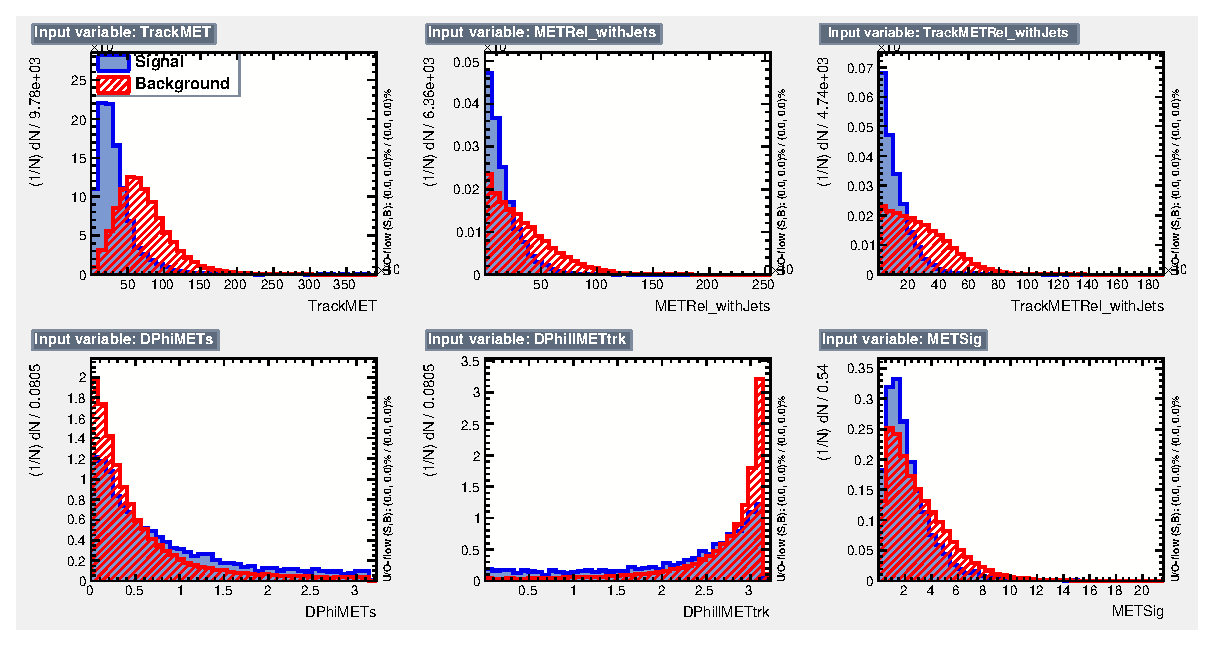
\includegraphics[width=0.45\linewidth]{Pictures/variables_id_c1.eps}
    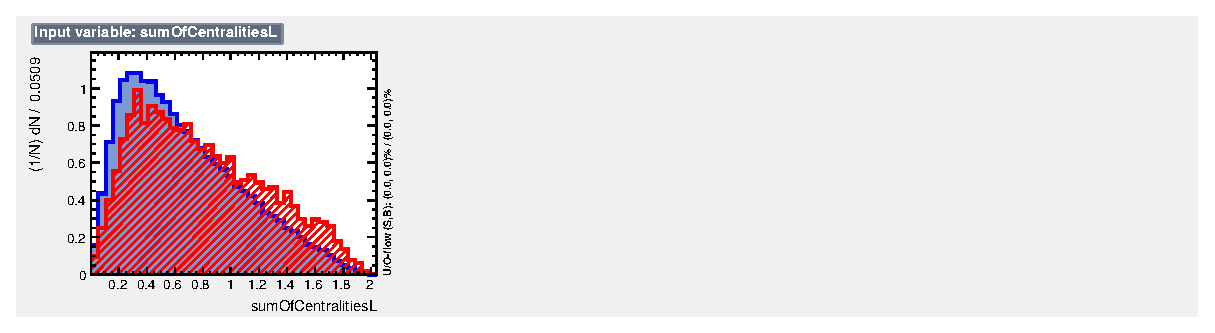
\includegraphics[width=0.45\linewidth]{Pictures/variables_id_c2.eps}
    \caption{Distributions of input variables to ggFCR1 BDT. Samples are unweighted and normalized to even numbers of background and signal events. Signal represents ggF and background all other samples.}.
    \label{fig:ggFCR1BDTinput}
\end{figure}
\begin{figure}[!htbp]
\centering
  \includegraphics[width=.4\linewidth]{Pictures/CorrelationMatrixS.eps}
  \includegraphics[width=.4\linewidth]{Pictures/CorrelationMatrixB.eps}
\caption{Correlations of input variables to ggFCR1 BDT. Signal represents ggF and background all other samples.}
\label{fig:ggFCR1corrSB}
\end{figure}

In order to quantify the discrimination we use the integrated-ROC calculated through TMVA for unweighted normalized samples and find an optimal value of 0.896. Comparisons between the test and training show that the BDT is un-biased- differences between testing and training samples would imply overtraining, or the BDT using to many parameters on too few events. Visually, once can see that the testing and trainings samples are quite similar. Additionally, a Kolmogorov-Smirnov test is performed to measure if the two test and training distributions differ significantly and no evidence of over-training is present. We can visualize the BDT output variable both on un-weighted normalized samples and on samples with all event weights applied. The following plots show BDT results applied to un-weighted and weighted samples.

\begin{figure}[!htbp]
\centering
  \includegraphics[width=.45\linewidth]{Pictures/overtrain_BDTG.eps}
  \includegraphics[width=.35\linewidth]{Pictures/run2-emme-CutVBFggFCR1-BDT_ggFCR1-log.pdf}
\caption{Unweighted, normalized samples of ggF (signal) and all other samples (background) plotted over BDT output distribution on left, overlaid testing and training samples shown. Right, full weighted samples of ggF signal and all other backgrounds plotted over BDT output distribution after ggF CR 1.}
\label{fig:ggFCR1BDTresult}
\end{figure}

\subsubsection{Discriminant in the GGF-CR2}

The multivariate discriminate used for the GGF CR2 is a boosted decision tree (BDT) trained using $e\mu+\mu e$ events that pass all ggF CR2 cuts. The training includes ggF events trained against VBF signal and all backgrounds. The MC statistics used in the training are half those available after ggF CR2 cuts (as the other half are later used to test the training). This corresponds to $\approx$ 3,200 ggF events and $\approx$480,000 other signal and background events.

The TMVA BDTG interface is used to train and test the BDT. The optimal parameters were found through a scan of reasonable values and the final set is summarized in Table~\ref{tab:ggFCR2BDTparameters}.
\begin{table}[h!]
\centering
\begin{tabular}{|l|c|c|}
\hline
Parameter                                    & Value     \\
\hline
Boosting algorithm                           & Gradient \\
Maximum tree depth                           &  10      \\
Number of trees                              &  100    \\
Minimum number of events requires per mode   &  5\%     \\ 
Number of cuts                               &  7       \\
\hline
\end{tabular}
\caption{BDT parameters used for the ggF CR2 training.}
\label{tab:ggFCR2BDTparameters}
\end{table}
For this BDT various distributions are used to take advantage of differences in distributions between ggF events and other sample types. These variables include $\Delta Y_{\ell\ell}$, $\Delta \Phi_{\ell\ell}$,$m_{\ell\ell}$,$m_T$,$p^T_{tot}$, lep $p^T_{\text{lead}}$, lep $p^T_{\text{sublead}}$, jet $p^T_{\text{lead}}$, jet $p^T_{\text{sublead}}$, $\Delta \Phi_{jj}$, and $\ensuremath{E_{\text{T,rel}}^{\text{miss}}}$. Distributions for these variables in the ggF CR2 region where the BDT is trained are shown below demonstrating data/MC modelling for each.
\begin{figure}[!h]
  \subfloat[$\Delta Y_{\ell\ell}$]{
      \includegraphics[width=0.3\textwidth]{Pictures/run2-emme-CutVBFggFCR2-DYll-log.pdf}
  }\hfill
  \subfloat[$\Delta \Phi_{\ell\ell}$]{
      \includegraphics[width=0.3\textwidth]{Pictures/run2-emme-CutVBFggFCR2-DPhill-log.pdf}
  }\hfill
  \subfloat[$m_{\ell\ell}$]{
      \includegraphics[width=0.3\textwidth]{Pictures/run2-emme-CutVBFggFCR2-Mll-log.pdf}
  }\hfill
  \subfloat[$m_T$]{
      \includegraphics[width=0.3\textwidth]{Pictures/run2-emme-CutVBFggFCR2-MT-log.pdf}
  }\hfill
  \subfloat[$p^T_{tot}$]{
      \includegraphics[width=0.3\textwidth]{Pictures/run2-emme-CutVBFggFCR2-PtTot-log.pdf}
  }\hfill
  \subfloat[lep $p^T_{\text{lead}}$]{
      \includegraphics[width=0.3\textwidth]{Pictures/run2-emme-CutVBFggFCR2-leadLepPt-log.pdf}
  }\hfill
  \subfloat[jet $p^T_{\text{lead}}$]{
      \includegraphics[width=0.3\textwidth]{Pictures/run2-emme-CutVBFggFCR2-leadJetPt-log.pdf}
  }\hfill
  \subfloat[lep $p^T_{\text{sublead}}$]{
      \includegraphics[width=0.3\textwidth]{Pictures/run2-emme-CutVBFggFCR2-subleadLepPt-log.pdf}
  }\hfill
  \subfloat[jet $p^T_{\text{sublead}}$]{
      \includegraphics[width=0.3\textwidth]{Pictures/run2-emme-CutVBFggFCR2-subleadJetPt-log.pdf}
  }\hfill
  \subfloat[$\Delta \Phi_{jj}$]{
      \includegraphics[width=0.3\textwidth]{Pictures/run2-emme-CutVBFggFCR2-DPhijj-log.pdf}
  }\hfill
  \subfloat[$\ensuremath{E_{\text{T,rel}}^{\text{miss}}}$]{
      \includegraphics[width=0.3\textwidth]{Pictures/run2-emme-CutVBFggFCR2-MET-log.pdf}
  }%\hfill
{\caption{Distributions of $\Delta Y_{\ell\ell}$, $\Delta \Phi_{\ell\ell}$,$m_{\ell\ell}$,$m_T$,$p^T_{tot}$, lep $p^T_{\text{lead}}$, lep $p^T_{\text{sublead}}$, jet $p^T_{\text{lead}}$, jet $p^T_{\text{sublead}}$, $\Delta \Phi_{jj}$, and $\ensuremath{E_{\text{T,rel}}^{\text{miss}}}$ in the ggF CR2 used as input to the BDT discriminating ggF from all other samples.
\label{fig:ggFCR2}}}
\end{figure} 

Plots shown in \ref{fig:ggFCR2BDTinput} and \ref{fig:ggFCR2corrSB} demonstrate the input distributions used to train the BDT and their correlations where each distribution is unweighted and normalized to equal number of background and signal events. 

\begin{figure}[!htbp]
    \centering
    \includegraphics[width=0.45\linewidth]{Pictures/variables_id_c1.eps}
    \includegraphics[width=0.45\linewidth]{Pictures/variables_id_c2.eps}
    \caption{Distributions of input variables to ggFCR2 BDT. Samples are unweighted and normalized to even numbers of background and signal events. Signal represents ggF and background all other samples.}.
    \label{fig:ggFCR2BDTinput}
\end{figure}
\begin{figure}[!htbp]
\centering
  \includegraphics[width=.4\linewidth]{Pictures/CorrelationMatrixS.eps}
  \includegraphics[width=.4\linewidth]{Pictures/CorrelationMatrixB.eps}
\caption{Correlations of input variables to ggFCR2 BDT. Signal represents ggF and background all other samples.}
\label{fig:ggFCR2corrSB}
\end{figure}

In order to quantify the discrimination we use the integrated-ROC calculated through TMVA for unweighted normalized samples and find an optimal value of 0.910. Comparisons between the test and training show that the BDT is un-biased- differences between testing and training samples would imply overtraining, or the BDT using to many parameters on too few events. Visually, once can see that the testing and trainings samples are quite similar. Additionally, a Kolmogorov-Smirnov test is performed to measure if the two test and training distributions differ significantly and no evidence of over-training is present. We can visualize the BDT output variable both on un-weighted normalized samples and on samples with all event weights applied. The following plots show BDT results applied to un-weighted and weighted samples.

\begin{figure}[!htbp]
\centering
  \includegraphics[width=.45\linewidth]{Pictures/overtrain_BDTG.eps}
  \includegraphics[width=.35\linewidth]{Pictures/run2-emme-CutVBFggFCR2-BDT_ggFCR2-log.pdf}
\caption{Unweighted, normalized samples of ggF (signal) and all other samples (background) plotted over BDT output distribution on left, overlaid testing and training samples shown. Right, full weighted samples of ggF signal and all other backgrounds plotted over BDT output distribution after ggF CR 2.}
\label{fig:ggFCR2BDTresult}
\end{figure}
\subsubsection{Discriminant in the GGF-CR3}

The multivariate discriminate used for the GGF CR3 is a boosted decision tree (BDT) trained using $e\mu+\mu e$ events that pass all ggF CR3 cuts. The training includes only ggF events trained against VBF signal and all backgrounds. The MC statistics used in the training are half those available after the ggF CR3 cuts (as the other half are later used to test the training). This corresponds to $\approx$ 3,200 ggF events and $\approx$480,000 other signal and background events.

The TMVA BDTG interface is used to train and test the BDT. The optimal parameters were found through a scan of reasonable values and the final set is summarized in Table~\ref{tab:ggFCR3BDTparameters}.
\begin{table}[h!]
\centering
\begin{tabular}{|l|c|c|}
\hline
Parameter                                    & Value     \\
\hline
Boosting algorithm                           & Gradient \\
Maximum tree depth                           &  10      \\
Number of trees                              &  1000    \\
Minimum number of events requires per mode   &  5\%     \\ 
Number of cuts                               &  7       \\
\hline
\end{tabular}
\caption{BDT parameters used for the ggF CR3 training.}
\label{tab:ggFCR3BDTparameters}
\end{table}
For this BDT various distributions are used to take advantage of differences in distributions between ggF events and other samples types. These variables include $\Delta Y_{\ell\ell}$, $\Delta \Phi_{\ell\ell}$,$m_{\ell\ell}$,$m_T$,$p^T_{tot}$, lep $p^T_{\text{lead}}$, lep $p^T_{\text{sublead}}$, and $\ensuremath{E_{\text{T}}^{\text{miss}}}$. Distributions for these variables in the ggF CR3 region where the BDT is trained are shown below demonstrating data/MC modelling for each.
\begin{figure}[!h]
  \subfloat[$\Delta Y_{\ell\ell}$]{
      \includegraphics[width=0.3\textwidth]{Pictures/run2-emme-CutVBFggFCR3_ZttBDT-DYll-log.pdf}
  }\hfill
  \subfloat[$\Delta \Phi_{\ell\ell}$]{
      \includegraphics[width=0.3\textwidth]{Pictures/run2-emme-CutVBFggFCR3_ZttBDT-DPhill-log.pdf}
  }\hfill
  \subfloat[$m_{\ell\ell}$]{
      \includegraphics[width=0.3\textwidth]{Pictures/run2-emme-CutVBFggFCR3_ZttBDT-Mll-log.pdf}
  }\hfill
  \subfloat[$m_T$]{
      \includegraphics[width=0.3\textwidth]{Pictures/run2-emme-CutVBFggFCR3_ZttBDT-MT-log.pdf}
  }\hfill
  \subfloat[$p^T_{tot}$]{
      \includegraphics[width=0.3\textwidth]{Pictures/run2-emme-CutVBFggFCR3_ZttBDT-PtTot-log.pdf}
  }\hfill
  \subfloat[lep $p^T_{\text{lead}}$]{
      \includegraphics[width=0.3\textwidth]{Pictures/run2-emme-CutVBFggFCR3_ZttBDT-leadLepPt-log.pdf}
  }\hfill
  \subfloat[lep $p^T_{\text{sublead}}$]{
      \includegraphics[width=0.3\textwidth]{Pictures/run2-emme-CutVBFggFCR3_ZttBDT-subleadLepPt-log.pdf}
  }\hfill
  \subfloat[$\ensuremath{E_{\text{T}}^{\text{miss}}}$]{
      \includegraphics[width=0.3\textwidth]{Pictures/run2-emme-CutVBFggFCR3_ZttBDT-MET-log.pdf}
  }\hfill
{\caption{Distributions of $\Delta Y_{\ell\ell}$, $\Delta \Phi_{\ell\ell}$,$m_{\ell\ell}$,$m_T$,$p^T_{tot}$, lep $p^T_{\text{lead}}$, lep $p^T_{\text{sublead}}$, and $\ensuremath{E_{\text{T}}^{\text{miss}}}$ in the ggF CR3 used as input to the BDT discriminating ggF from all other samples.
\label{fig:ggFCR3}}}
\end{figure} 

Plots shown in \ref{fig:ggFCR3BDTinput} and \ref{fig:ggFCR3corrSB} demonstrate the input distributions used to train the BDT and their correlations where each distribution is unweighted and normalized to equal number of background and signal events. 

\begin{figure}[!htbp]
    \centering
    \includegraphics[width=0.45\linewidth]{Pictures/variables_id_c1.eps}
    \includegraphics[width=0.45\linewidth]{Pictures/variables_id_c2.eps}
    \caption{Distributions of input variables to ggFCR3 BDT. Samples are unweighted and normalized to even numbers of background and signal events. Signal represents ggF and background all other samples.}.
    \label{fig:ggFCR3BDTinput}
\end{figure}
\begin{figure}[!htbp]
\centering
  \includegraphics[width=.4\linewidth]{Pictures/CorrelationMatrixS.eps}
  \includegraphics[width=.4\linewidth]{Pictures/CorrelationMatrixB.eps}
\caption{Correlations of input variables to ggFCR3 BDT. Signal represents ggF and background all other samples.}
\label{fig:ggFCR3corrSB}
\end{figure}

In order to quantify the discrimination we use the integrated-ROC calculated through TMVA for unweighted normalized samples and find an optimal value of 0.901. Comparisons between the test and training show that the BDT is un-biased- differences between testing and training samples would imply overtraining, or the BDT using to many parameters on too few events. Visually, once can see that the testing and trainings samples are quite similar. Additionally, a Kolmogorov-Smirnov test is performed to measure if the two test and training distributions differ significantly and no evidence of over-training is present. We can visualize the BDT output variable both on un-weighted normalized samples and on samples with all event weights applied. The following plots show BDT results applied to un-weighted and weighted samples.

\begin{figure}[!htbp]
\centering
  \includegraphics[width=.45\linewidth]{Pictures/overtrain_BDTG.eps}
  \includegraphics[width=.35\linewidth]{Pictures/run2-emme-CutVBFggFCR3_ZttBDT-BDT_ggFCR3-log.pdf}
\caption{Unweighted, normalized samples of ggF (signal) and all other samples (background) plotted over BDT output distribution on left, overlaid testing and training samples shown. Right, full weighted samples of ggF signal and all other backgrounds plotted over BDT output distribution after ggF CR 3.}
\label{fig:ggFCR3BDTresult}
\end{figure}

\subsubsection{Dependance on the modelling of the simulation} 

This method detetextines $gg$F the background entirely from data and, thus, the sensitivity to migration of events from one region to the other is greatly reduced. In order to study this, pseudo-experiments were thrown using Asimov data-sets. For each toy set the input yield for for each region was varied independently in the range of $0<\mu_{\text{GGF-X}}<2$ at generation level. The measured variation of the VBF yield in the signal region with respect to the nominal conditions corresponds to the sensitivity to event-migration across categories in simulation due to systematic uncertainties in the predictions. 


\begin{table}
\centering
\begin{tabular}{l c c c c}
Param name & Patextam Val &  $\Delta{ggFCRNj1}$ & $\Delta{ggFCRNj2}$ & $\Delta{ggFCRNj3}$ \\
$\mu_{\text VBF}$ &  $1.00^{+0.36}_{-0.33}$ & 0.10 & 0.10 & 0.10 \\ 
$\mu_{\text VBF}$ &  $1.00^{+0.34}_{-0.31}$ & 0.10 & 0.10 & 0.50 \\ 
$\mu_{\text VBF}$ &  $1.00^{+0.33}_{-0.30}$ & 0.10 & 0.10 & 1.00 \\ 
$\mu_{\text VBF}$ &  $1.00^{+0.36}_{-0.33}$ & 0.10 & 0.50 & 0.10 \\ 
$\mu_{\text VBF}$ &  $1.00^{+0.34}_{-0.31}$ & 0.10 & 0.50 & 0.50 \\ 
$\mu_{\text VBF}$ &  $1.00^{+0.33}_{-0.30}$ & 0.10 & 0.50 & 1.00 \\ 
$\mu_{\text VBF}$ &  $1.00^{+0.36}_{-0.33}$ & 0.10 & 1.00 & 0.10 \\ 
$\mu_{\text VBF}$&  $1.00^{+0.34}_{-0.31}$ & 0.10 & 1.00 & 0.50 \\ 
$\mu_{\text VBF}$&  $1.00^{+0.33}_{-0.30}$ & 0.10 & 1.00 & 1.00 \\ 
$\mu_{\text VBF}$&  $1.00^{+0.36}_{-0.33}$ & 0.50 & 0.10 & 0.10 \\ 
$\mu_{\text VBF}$&  $1.00^{+0.34}_{-0.31}$ & 0.50 & 0.10 & 0.50 \\ 
$\mu_{\text VBF}$&  $1.00^{+0.33}_{-0.30}$ & 0.50 & 0.10 & 1.00 \\ 
$\mu_{\text VBF}$&  $1.00^{+0.36}_{-0.33}$ & 0.50 & 0.50 & 0.10 \\ 
$\mu_{\text VBF}$&  $1.00^{+0.34}_{-0.31}$ & 0.50 & 0.50 & 0.50 \\ 
$\mu_{\text VBF}$&  $1.00^{+0.33}_{-0.30}$ & 0.50 & 0.50 & 1.00 \\ 
$\mu_{\text VBF}$&  $1.00^{+0.36}_{-0.33}$ & 0.50 & 1.00 & 0.10 \\ 
$\mu_{\text VBF}$&  $1.00^{+0.34}_{-0.31}$ & 0.50 & 1.00 & 0.50 \\ 
$\mu_{\text VBF}$&  $1.00^{+0.33}_{-0.30}$ & 0.50 & 1.00 & 1.00 \\ 
$\mu_{\text VBF}$&  $1.00^{+0.36}_{-0.33}$ & 1.00 & 0.10 & 0.10 \\ 
$\mu_{\text VBF}$&  $1.00^{+0.34}_{-0.31}$ & 1.00 & 0.10 & 0.50 \\ 
$\mu_{\text VBF}$&  $1.00^{+0.33}_{-0.30}$ & 1.00 & 0.10 & 1.00 \\ 
$\mu_{\text VBF}$&  $1.00^{+0.36}_{-0.33}$ & 1.00 & 0.50 & 0.10 \\ 
$\mu_{\text VBF}$&  $1.00^{+0.34}_{-0.31}$ & 1.00 & 0.50 & 0.50 \\ 
$\mu_{\text VBF}$&  $1.00^{+0.33}_{-0.30}$ & 1.00 & 0.50 & 1.00 \\ 
$\mu_{\text VBF}$&  $1.00^{+0.36}_{-0.33}$ & 1.00 & 1.00 & 0.10 \\ 
$\mu_{\text VBF}$&  $1.00^{+0.34}_{-0.31}$ & 1.00 & 1.00 & 0.50 \\ 
$\mu_{\text VBF}$&  $1.00^{+0.33}_{-0.30}$ & 1.00 & 1.00 & 1.00 \\ 
\end{tabular}
\label{tab:ggFBias}
\end{table}

\subsection{Fake backgrounds}
The final substantial background in the VBF HWW differential coupling analysis comes from mis-identified leptons. These are jets that are mistakenly identified as leptons in reconstruction and in this analysis these predominantly come from $W+$jet events. In these events a $W$ boson decays leptonically leading to one true lepton and a jet from the primary vertex is mistaken for a lepton. This creates an event which mimics our desired two lepton signature and so creates an additional HWW background sample. This background is estimated as in the HWW coupling analysis using the fake factor method, similarly to in the 2016 HWW coupling analysis. Further detail on the overall fake factor method and its mathematical formulation can be found here \cite{fakesfactormethod} while further details on HWW-specific fake background studies are here \cite{HWWCoupling}. In this section I will give a brief summary of fake estimations along with the slightly augmented fake factor control region definition used in the HWW differential coupling analysis. 

The fake background is estimated using data which is measured in a region defined by signal region cuts with one important distinction- one or both of the leptons used are ``anti-identified'' meaning they pass some looser lepton identification criteria but not the one used in the analysis signal region. These fakes are then extrapolated to the true signal region (with two ``identified'' electrons fake factors. Fake factors are measured as functions of $p_T$ and $\eta$ in jet-enriched $Z+$jets samples and are defined as the ratio of identified to anti-identified leptons. The fake backgrounds can be considered split between ``single-fake'' (with one ``anti-ID'' lepton) from the predominant $W+$jets background and ``double-fake'' (with two ``anti-ID'' leptons from QCD processes. The total signal sample can be defined as: 
\begin{equation}
N_{id+id} = N^{EW}_{id+id}+N^{W+jets}_{id+id}+N^{QCD}_{id+id}
\end{equation} 
so that the total events include all electroweak processes ($N^{EW}_{id+id}$) as well as fake backgrounds from $W+$jets and QCD events. In order to estimate the total fake background in the signal region we need to estimate the number of $W+$jets and QCD events in ``id+anti-id'' events and then apply the fake factor to extrapolate into the ``id+id'' region. The $N_{id+anti-id}$ for fake backgrounds is calculated after subtraction of electroweak backgrounds (two true leptons that contaminate the ``id+anti-id region'') from Monte Carlo simulations as follows:
\begin{equation}
N^{W+jets}_{id+anti-id}+N^{QCD}_{id+anti-id}=N_{id+anti-id}-N^{EW MC}_{id+anti-id}
\end{equation}
 
Fake factors are derived from $Z+$jets samples and then applied to $W+$jets regions so the differences between these two samples are important to uncderstand fully. The fake factor is defined 
\begin{equation}
F.F. = \frac{N_{id}}{N_{anti-id}}
\end{equation}
and is measured separately for electron and muons and measured in bins of $\eta$ and $p_T$. The following table summarizes to ``id'' and ``anti-id'' requirements. 

\begin{table}[tb]
\caption{Requirements for ``identified'' and ``anti-identified'' electrons and muons.}
\label{tab:idantiid}
\scalebox{0.7}{
\centering
\begin{tabular}{c|c||c|c}
  \hline
  ``id'' electron & ``anti-id'' electron & ``id'' muon & ``anti-id'' muon   \\
  \hline
  \multicolumn{2}{c|}{\centering $p_T>15$ GeV} & \multicolumn{2}{l|}{\centering $p_T>15$ GeV} \\
  \multicolumn{2}{c|}{\centering $|\eta| <$2.47, excluding 1.37$<|\eta|<$1.52} & \multicolumn{2}{c|}{\centering $|\eta|<$2.45} \\
  \multicolumn{2}{c|}{\centering $|z_0$sin$\theta|<$ 0.5mm} & \multicolumn{2}{c|}{\centering $|z_0$sin$\theta|<$ 0.5mm} \\
  Pass \textit{Tight} if $p_T<25$ GeV & \multirow{2}{*}{ \centering Pass \textit{Loose}} & \multirow{2}{*}{ \centering Pass \textit{Tight}} & \multirow{2}{*}{\centering Pass \textit{Medium}} \\
  Pass \textit{Medium} if $p_T>25$ GeV & & & \\
  \multicolumn{2}{c|}{\centering $|d_0|\sigma(d_0)<5$} & $|d_0|\sigma(d_0)<3$ & $|d_0|\sigma(d_0)<15$ \\
  Pass FixedCutTrackCone40 if $p_T<25$GeV & & $E_T^{cone20}/p_T < 0.09$ & \\
  Pass IsoGradient if $p_T<25$GeV & & $p_T^{varcone30}/p_T<0.06$ & \\
   & Veto against identified electron & & Veto against identified muon \\
\hline
\hline
\end{tabular}
}
\end{table}
$Z+$jets event are selected to contain exactly three loosely identified leptons with $p_T>15$GeV. Further requirements are for an opposite sign $ee$ or $\mu\mu$ lepton pair with 7-GeV$< m_{\ell\ell} < 110$GeV. Both $Z$ candidate leptons must be ``identified'' so that the third is the fake candidate. An additional $WZ$ veto is applied using $m_T>50$GeV to mitigate electroweak background in the $Z+$jets sample. Dedicated MC model electroweak backgrounds in the $Z+$jets region and include $V+\gamma$, diboson ($WW$, $WZ$, and $ZZ$), single top and $t\bar{t}$. Finally, $WZ$ backgrounds are normalized ot their measured cross-sections. Fake yields for the $Z+$jets samples are finally calculated by subtracting data from all MC electroweak backgrounds. The $Z+$jets cutflow for fake estimation in the $ee+\mu\mu$ channel is shown next. 

\textcolor{red}{Add Z+jets cutflow and plots?}

The fake factor is computed as a binned ratio in $p_T$, $[15,20,25,35,\inf]$ and for muons also in $\eta$ for $[0,1.5,2.5]$ exluding the electromagnetic calorimeter crack region. The following table summarized fake factors used in this analysis.

\begin{table}[tb]
\centering
\caption{Fake factors binned for muons and electrons in $p_T$ and $\eta$ with their statistical uncertainties}
\label{tab:FakeFactors}
\begin{tabular}{c|c|c|c}
$p_T$(GeV) & Muon FF ($|\eta|<1.5$) & Muon FF ($1.5<|\eta|<2.5$) & Electron FF \\
\hline
15-25 & 0.038$\pm$ 0.004 & 0.057$\pm$0.005 & 0.079$\pm$0.005 \\
20-25 & 0.021$\pm$ 0.007 & 0.0357$\pm$0.0077 & 0.097$\pm$0.001 \\
25-35 & 0.029$\pm$ 0.011 & 0.064$\pm$0.014 & 0.157$\pm$0.017 \\
35-$\inf$ & 0.049$\pm$ 0.023 & 0.11$\pm$0.04 & 0.19$\pm$0.026 \\
\end{tabular}
\end{table}

Further studies on fake factors include comparisons to their MC simulation expectations and studies on differences between the $Z+$jets control sample used to calculate fake factors and the $W+$jets sample on which they are applied. These studies are beyond the scope of this thesis but support the use of the fake factor method in our analysis. Specifically, jet kinematics and heavy flavor fraction in both samples are have been studied by the HWW coupling analysis and factor into a correction factor applied to transfer between $Z+$jets and $W+$jets samples. More information on these studies and correction factors can be found in \cite{HWWCoupling}. 

The $W+$jets control region is defined as in the signal region, with cuts specifying at least 2 jets, a $b$-veto, $m_{\tau\tau}$ based Z-veto, an opposite lepton veto, central jet veto, and cuts on $m_{jj}$ and $\Delta Y_{jj}$. Unlike the signal region, this region also specified one ``id'' and one ``anti-id'' lepton instead of two identified leptons. The cutflow for this region is shown below where fakes are defined from the subtraction of total electroweak background from data. Fake purity in this control region is $74\%$ after all signal region-like cuts are applied.

\begin{table}[h!]
\scalebox{0.6}{
%%% created on Mon Apr 20 12:30:43 2020 from TQSampleFolder 'samples' with TQLibrary UNKNOWN compiled with GCC 8.3.0 against ROOT 6.16/00
\providecommand{\xmark}{{\sffamily \bfseries X}}
\providecommand\rotatecell[2]{\rotatebox[origin=c]{#1}{#2}}
\begin{tabular}{ c || c | c | c  c }
\ensuremath{\sqrt{s}=13 TeV}, \ensuremath{\mathcal{L}=139 fb^{-1}}  (Full~Run~2) & Total Bkg & Data & Fakes & Fake purity(\%)\tabularnewline
\hline
Channel Selection & \ensuremath{8116768.84\pm 3042.09} & \ensuremath{13124937} & \ensuremath{5008168.16\pm 4730.67} & \ensuremath{38.16\pm 0.04}\tabularnewline
Trigger Selection & \ensuremath{8116768.84\pm 3042.09} & \ensuremath{13124937} & \ensuremath{5008168.16\pm 4730.67} & \ensuremath{38.16\pm 0.04}\tabularnewline
Trigger Matching & \ensuremath{7906126.65\pm 2917.00} & \ensuremath{13057932} & \ensuremath{5151805.35\pm 4644.01} & \ensuremath{39.45\pm 0.04}\tabularnewline
W+jets flavour split muon & \ensuremath{5896841.78\pm 2703.75} & \ensuremath{10572340} & \ensuremath{4675498.22\pm 4228.78} & \ensuremath{44.22\pm 0.04}\tabularnewline
W+jets flavour split electron & \ensuremath{3791849.84\pm 2494.76} & \ensuremath{7417426} & \ensuremath{3625576.16\pm 3693.41} & \ensuremath{48.88\pm 0.05}\tabularnewline
Jet Cleaning & \ensuremath{3791849.84\pm 2494.76} & \ensuremath{7417426} & \ensuremath{3625576.16\pm 3693.41} & \ensuremath{48.88\pm 0.05}\tabularnewline
Overlap: Vgamma/Vjets & \ensuremath{3791849.84\pm 2494.76} & \ensuremath{7417426} & \ensuremath{3625576.16\pm 3693.41} & \ensuremath{48.88\pm 0.05}\tabularnewline
Only two Leptons & \ensuremath{3754720.02\pm 2485.95} & \ensuremath{7376514} & \ensuremath{3621793.98\pm 3681.91} & \ensuremath{49.10\pm 0.05}\tabularnewline
$p_{t}^{lead} > 22$ GeV & \ensuremath{3754720.02\pm 2485.95} & \ensuremath{7376514} & \ensuremath{3621793.98\pm 3681.91} & \ensuremath{49.10\pm 0.05}\tabularnewline
$p_{t}^{\rm sublead} > 15$ & \ensuremath{3753322.61\pm 2485.49} & \ensuremath{7373346} & \ensuremath{3620023.39\pm 3681.17} & \ensuremath{49.10\pm 0.05}\tabularnewline
OS Leptons & \ensuremath{3751223.46\pm 2483.45} & \ensuremath{7365693} & \ensuremath{3614469.54\pm 3678.75} & \ensuremath{49.07\pm 0.05}\tabularnewline
$M_{\ell\ell} > 12/10$ GeV & \ensuremath{3751147.28\pm 2483.41} & \ensuremath{7365336} & \ensuremath{3614188.72\pm 3678.68} & \ensuremath{49.07\pm 0.05}\tabularnewline
SF: Z Veto & \ensuremath{3751147.28\pm 2483.41} & \ensuremath{7365336} & \ensuremath{3614188.72\pm 3678.68} & \ensuremath{49.07\pm 0.05}\tabularnewline
Leptons ID-anti-ID & \ensuremath{780838.94\pm 837.46} & \ensuremath{1931616} & \ensuremath{1150777.06\pm 1622.64} & \ensuremath{59.58\pm 0.09}\tabularnewline
\hline
2-jet (30,30) fJVT & \ensuremath{384692.76\pm 242.92} & \ensuremath{657536} & \ensuremath{272843.24\pm 846.49} & \ensuremath{41.49\pm 0.14}\tabularnewline
b-veto & \ensuremath{62361.10\pm 199.23} & \ensuremath{198158} & \ensuremath{135796.90\pm 487.70} & \ensuremath{68.53\pm 0.29}\tabularnewline
CJV (20GeV) & \ensuremath{43093.51\pm 171.93} & \ensuremath{137885} & \ensuremath{94791.49\pm 409.20} & \ensuremath{68.75\pm 0.35}\tabularnewline
OLV bool & \ensuremath{9162.00\pm 78.28} & \ensuremath{28068} & \ensuremath{18906.00\pm 184.92} & \ensuremath{67.36\pm 0.77}\tabularnewline
$Z\to\tau\tau$ veto & \ensuremath{5142.69\pm 60.99} & \ensuremath{18069} & \ensuremath{12926.31\pm 147.61} & \ensuremath{71.54\pm 0.97}\tabularnewline
$M_{jj}>$200 & \ensuremath{3233.48\pm 51.55} & \ensuremath{11911} & \ensuremath{8677.52\pm 120.70} & \ensuremath{72.85\pm 1.21}\tabularnewline
$DY_{jj}>$2.1 & \ensuremath{2838.02\pm 50.56} & \ensuremath{10904} & \ensuremath{8065.98\pm 116.02} & \ensuremath{73.97\pm 1.28}\tabularnewline
\end{tabular}

}
\caption{Cutflow in the fakes control region.}
\label{tab:fakescr}
\end{table}

Distributions below show the electroweak background processes (blue) in the fake control region along with data (black). The $W+$jets or fake background is taken as the difference between data and EW background and shown in the plots as light blue points. High fake purity is shown and these backgrounds are used along with fake factors to estimate fakes in contaminating our signal region.

\begin{figure}[!h]
  \subfloat[$p_T^{\ell\ell}$]{
      \includegraphics[width=0.3\textwidth]{Pictures/run2-emme-CutVBFWCRDYjjMin-Ptll-log.pdf}
  }\hfill
%  \subfloat[$\Delta \Phi_{\ell\ell}$]{
%      \includegraphics[width=0.3\textwidth]{Pictures/run2-emme-CutVBFWCRDYjjMin-DPhill-log.pdf}
%  }\hfill
  \subfloat[$m_{\ell\ell}$]{
      \includegraphics[width=0.3\textwidth]{Pictures/run2-emme-CutVBFWCRDYjjMin-Mll-log.pdf}
  }\hfill
  \subfloat[$m_T$]{
      \includegraphics[width=0.3\textwidth]{Pictures/run2-emme-CutVBFWCRDYjjMin-MT-log.pdf}
  }\hfill
  \subfloat[$p^T_{tot}$]{
      \includegraphics[width=0.3\textwidth]{Pictures/run2-emme-CutVBFWCRDYjjMin-PtTot-log.pdf}
  }\hfill
  \subfloat[lep $p^T_{\text{lead}}$]{
      \includegraphics[width=0.3\textwidth]{Pictures/run2-emme-CutVBFWCRDYjjMin-leadLepPt-log.pdf}
  }\hfill
%  \subfloat[jet $p^T_{\text{lead}}$]{
%      \includegraphics[width=0.3\textwidth]{Pictures/run2-emme-CutVBFWCRDYjjMin-leadJetPt-log.pdf}
%  }\hfill
%  \subfloat[lep $p^T_{\text{sublead}}$]{
%      \includegraphics[width=0.3\textwidth]{Pictures/run2-emme-CutVBFWCRDYjjMin-subleadLepPt-log.pdf}
%  }\hfill
%  \subfloat[jet $p^T_{\text{sublead}}$]{
%      \includegraphics[width=0.3\textwidth]{Pictures/run2-emme-CutVBFWCRDYjjMin-subleadJetPt-log.pdf}
%  }\hfill
  \subfloat[$m_{jj}$]{
      \includegraphics[width=0.3\textwidth]{Pictures/run2-emme-CutVBFWCRDYjjMin-Mjj-log.pdf}
  }\hfill
  \subfloat[$\ensuremath{E_{\text{T,rel}}^{\text{miss}}}$]{
      \includegraphics[width=0.3\textwidth]{Pictures/run2-emme-CutVBFWCRDYjjMin-MET-log.pdf}
  }%\hfill
{\caption{Distributions of $p_T^{\ell\ell}$, $m_{\ell\ell}$,$m_T$,$p^T_{tot}$, lep $p^T_{\text{lead}}$, lep $p^T_{\text{sublead}}$, $m_{jj}$, and $\ensuremath{E_{\text{T,rel}}^{\text{miss}}}$ in the differential VBF $W+$jets control region.
\label{fig:WCR}}}
\end{figure}  

The EW background subtracted from data in the $W+$jets control region consists of $V\gamma$, diboson, top, and $Z+$jets events. \textcolor{red}{Add a breakdown of EW background types in plots and cutflows?}

\section{Systematic uncertainties}
The experimental, theoretical, and statistical uncertainties in this analysis all impact the final measurement substantially. In this section I describe first the experimental systematic uncertainties then the theoretical in detail. Statistical uncertainties are derived from the limited number of MC events used to model each of signal and background samples per bin in the differential measurement. A single MC-stat nuisance parameter is implemented based on Poisson statistics and used in our overal statistical fit. 

\subsection{Experimental uncertainties}
Several types of experimental systematics uncertainties affect this analysis. Each of these are calculated for this analysis using the current recommendations for each of the following Combined Performance groups: muons, electrons, Jet/$E_T^{miss}$, Trigger, flavor tagging (?), and pile-up. The current set of experimental systematics uses 102 nuisance parameters, each of which will be briefly described next.
 
There are two different ways systematic uncertainties are calculated and applied. First, for systematic uncertainties on the energy of jets and electrons and momentum of muons, the scale and resolutions is calculated. These test the number of events in the final state affected by shifting energy/momentum by a scale factor. This ``smearing'' procedure is done for a nominal scaling value and values with $\pm 1 \sigma$. Next, systematic uncertainty on the scale factors is calculated by comparing nominal event numbers to those after particular weights are applied. These weights are derived from data-MC agreement and their uncertainty is the relative difference between nominal and modified weight sums.  
 
At the end of this section there is a table which describes all key experimental uncertainties and then tables of experimental uncertainties in the signal region, $Z\rightarrow \tau\tau$ and top control regions are shown. \textcolor{red}{Not included yet are shape systematics on the BDT distribution are also considered for all the experimental systematic uncertanties, maybe necessary, and acceptance in the signal region, $Z\rightarrow\tau\tau$ and top control regions.}
\\
\textbf{Muon reconstruction and identification}
There are four nuisance parameters associated with muon reconstruction and identification, these are reconstruction efficiency statistic and systematic uncertainties ($MUON\_EFF\_RECO\_STAT$, $MUON\_EFF\_RECO\_SYS$). There are additional separate uncertainties for low $p_T$ muons, or those with $3 < p_T <20$ GeV ($MUON\_EFF\_RECO\_STAT\_LOWPT$, $MUON\_EFF\_RECO\_SYS\_LOWPT$).

\textbf{Muon momentum scale and resolution}
Muon momentum resolution uncertainties are divided into those from the Inner Detector ($MUON\_ID$) and those from the muon spectrometer ($MUON\_MS$). Muon momentum scale uncertainties are contained in $MUON\_SCALE$. Finally, two additional systematic uncertainties $MUON\_SAGITTA\_RESBIAS$ and $MUON\_SAGITTA\_RHO$ come from a correction applied to muons to account for residual ID/MS misalignments which create a charge dependent bias.  

\textbf{Electron reconstruction and identification}
lectron reconstruction and identification uncertainties come from nuisance parameters $EL\_EFF\_Reco\_TOTAL\_1NPCOR\_PLUS\_UNCOR$,$EL\_EFF\_ID\_CorrUncertaintyNP$ 0 to 15, and $EL\_EFF\_ID\_SIMPLIFIED\_UncorrUncertaintyNP$ 0 to 17.

\textbf{Electron energy scale and resolution}
The standard systematics included for electron energy scale and resolution are $EG\_SCALE\_AF2$ and $EG\_SCALE\_ALL$.\textcolor{red}{Missing resolution NP?}

\textbf{Jet energy scale and resolution}
There are a number of jet energy scale and resolution systematics included in the analysis: $JET\_BJES\_Response$,$JET\_EffectiveNP\_Detector$ 1 to 2, $JET\_EffectiveNP\_Mixed$ 1 to 3, $JET\_EffectiveNP\_Modelling$ 1 to 4, $JET\_EffectiveNP\_Statistical$ 1 to 6, $JET\_EtaIntercalibration\_Modelling$, $JET\_EtaIntercalibration\_NonClosure\_highE$, $JET\_EtaIntercalibration\_NonClosure\_negEta$, $JET\_EtaIntercalibration\_NonClosure\_posEta$, $JET\_EtaIntercalibration\_TotalStat$, $JET\_Flavor\_Composition$, $JET\_Flavor\_Response$, $JET\_JER\_DataVsMC$, $JET\_JER\_EffectiveNP\_$ 1 to 7, $JET\_JvtEfficiency$, $JET\_PunchThrough\_MC16$, $JET\_SingleParticle\_HighPt$.

\textbf{Isolation}
One isolation systematic uncertainty included is for electrons ($EL\_EFF\_Iso\_TOTAL\_1NPCOR\_PLUS\_UNCOR$) and \textcolor{red}{another two are included for muons:$MUON\_ISO\_STAT$ and $MUON\_ISO\_SYS$ . These aren't included currently?}

\textbf{Trigger efficiency}
Three nuisance parameters are included for trigger efficiency- one for electrons ($EL\_EFF\_Trigger\_TOTAL\_1NPCOR\_PLUS\_UNCOR$) and two for muons ($MUON\_EFF\_TrigStatUncertainty$ and $MUON\_EFF\_TrigSystUncertainty$) \textcolor{red}{Muon Syst isn't included...}.

\textbf{Flavor tagging efficiency}
Flavor tagging efficiency nuisance parameters considered are $FT\_EFF\_Eigen\_B\_$ 0 to 2, $FT\_EFF\_Eigen\_C\_$ 0 to 2, $FT\_EFF\_Eigen\_Light\_$ 0 to 3, $FT\_EFF\_extrapolation$, and $FT\_EFF\_extrapolation\_from\_charm$.

\textbf{Pileup reweighting and integrated luminosity}
The data scale factor for the pileup $<\mu>$ value is $1.0/1.09$ \textcolor{red}{Update this value?}. Systematics of the pileup $<\mu>$ value are accounted for with the nuisance parameter $PRW\_DATASF$ and evaluated by varying the data scale factor upward and downward. Jet pileup nuisance parameters are also included: $JET\_Pileup\_OffsetMu$,$JET\_Pileup\_OffsetNPV$, $JET\_Pileup\_PtTerm$, amd $JET\_Pileup\_RhoTopology$.

\textbf{Integrated luminosity}
Uncertainty on the integrated luminosity is $\pm 2.1\%$ for the 2015$+$2016 dataset, $\pm 2.4\%$ for the 2017 dataset and $\pm 2.0\%$ for the 2018 dataset. This results in an overall integrated luminosity uncertainty of $\pm 1.7\%$ ~\cite{ATLAS-CONF-2019-021}.

\begin{table}
\resizebox{\textwidth}{!}{
  \begin{tabular}{l|l}
  \hline\hline
  Systematic uncertainty & Short description \\
  \hline
  \multicolumn{2}{c}{Event}\\
  \hline
  Luminosity         & uncertainty on total integrated luminosity \\
  PRW\_DATASF	     & uncertainty on pileup reweighting          \\
  \hline
  \multicolumn{2}{c}{Electrons}\\
  \hline
  EL\_EFF\_Trigger\_Total\_1NPCOR\_PLUS\_UNCOR            &  trigger efficiency uncertainty          \\
  EL\_EFF\_Reco\_Total\_1NPCOR\_PLUS\_UNCOR               &  reconstruction efficiency uncertainty   \\
  EL\_EFF\_ID\_CorrUncertaintyNP (0 to 15)                &  ID efficiency uncertainty splits in 16 components   \\
  EL\_EFF\_ID\_SIMPLIFIED\_UncorrUncertaintyNP (0 to 17)  &  ID efficiency uncertainty splits in 18 components   \\
  EL\_EFF\_Iso\_Total\_1NPCOR\_PLUS\_UNCOR                &  isolation efficiency uncertainty        \\
  EG\_SCALE\_ALL                                          &\multirow{2}{*}{energy scale uncertainty} \\
  EG\_SCALE\_AF2	                                  &                                          \\
 % EG\_RESOLUTION\_ALL                                     &  energy resolution uncertainty           \\
  \hline
  \multicolumn{2}{c}{Muons}\\
  \hline
  MUON\_EFF\_TrigStatUncertainty &  \multirow{2}{*}{trigger efficiency uncertainty} \\
% MUON\_EFF\_TrigSystUncertainty &                                                  \\
  MUON\_EFF\_STAT                &  \multirow{2}{*}{reconstruction and ID efficiency uncertainty for muons with $p_T$ > 20 GeV} \\
  MUON\_EFF\_SYS                 &                                                                      \\
  MUON\_EFF\_STAT\_LOWPT         & \multirow{2}{*}{reconstruction and ID efficiency uncertainty for muons with $p_T$ < 20 GeV} \\
  MUON\_EFF\_SYST\_LOWPT         &                                                                      \\
% MUON\_ISO\_STAT                &  \multirow{2}{*}{isolation efficiency uncertainty}                   \\
% MUON\_ISO\_SYS                 &                                                                      \\
% MUON\_TTVA\_STAT               &  \multirow{2}{*}{track-to-vertex association efficiency uncertainty} \\
% MUON\_TTVA\_SYS                &                                                                      \\
  MUON\_ID                       & momentum resolution uncertainty from inner detector                  \\
  MUON\_MS                       & momentum resolution uncertainty from muon system                     \\
  MUON\_SCALE                    & momentum scale uncertainty                                           \\
  MUON\_SAGITTA\_RHO             & \multirow{2}{*}{charge dependent momentum scale uncertainty}         \\
  MUON\_SAGITTA\_RESBIAS         &                                                                      \\
  \hline
  \multicolumn{2}{c}{Jets}\\
  \hline         
  JET\_EffectiveNP\_Detector (1 to 2) & detector related energy scale uncertainty \\
  JET\_JER\_EffectiveNP\_ (1 to 7) & energy resolution uncertainty  \\
  JET\_JER\_DataVsMC 	& energy resolution modelling uncertainty \\
  JET\_BJES\_Response & energy scale uncertainty on b-jets \\
  JET\_EffectiveNP\_Mixed (1 to 3) & energy resolution uncertainty \\
  JET\_EffectiveNP\_Modelling (1 to 4) &  energy scale uncertainty on eta-intercalibration (modeling) \\
  JET\_EffectiveNP\_Statistical (1 to 6) &  statistical resolution uncertainty \\
  JET\_EtaIntercalibration\_NonClosure\_negEta &  energy scale uncertainty on eta-intercalibrations (non-closure) \\
  JET\_EtaIntercalibration\_NonClosure\_posEta & energy scale uncertainty on eta-intercalibrations (non-closure) \\
  JET\_EtaIntercalibration\_TotalStat & energy scale uncertainty on eta-intercalibrations (statistics/method) \\
  JET\_Pileup\_OffsetMu                & energy scale uncertainty on pile-up (mu dependent)    \\
  JET\_Pileup\_OffsetNPV               & energy scale uncertainty on pile-up (NPV dependent)   \\
  JET\_Pileup\_PtTerm                  & energy scale uncertainty on pile-up (pt term)         \\
  JET\_Pileup\_RhoTopology             & energy scale uncertainty on pile-up (density $\rho$)  \\
  JET\_Flavor\_Composition             & energy scale uncertainty on flavour composition       \\
  JET\_Flavor\_Response                & energy scale uncertainty on samples' flavour response \\
  JET\_PunchThrough\_MC16              & energy scale uncertainty for punch-through jets       \\
  JET\_SingleParticle\_HighPt          & energy scale uncertainty from the behaviour of high-$p_T$ jets \\
  JET\_JvtEfficiency & JVT efficiency uncertainty      \\
  FT\_EFF\_Eigen\_B (0 to 2) & \multirow{3}{*}{\parbox{11cm}{$b$-tagging efficiency uncertainties (``BTAG\_MEDIUM''): 3 components for $b$ jets, 3 for $c$ jets and 4 for light jets}} \\
  FT\_EFF\_Eigen\_C (0 to 2)                 & \\
  FT\_EFF\_Eigen\_Light (0 to 3)             & \\
  FT\_EFF\_Eigen\_extrapolation              & $b$-tagging efficiency uncertainty on the extrapolation to high-$p_T$ jets\\
  FT\_EFF\_Eigen\_extrapolation\_from\_charm & $b$-tagging efficiency uncertainty on tau jets \\
\hline\hline     
\end{tabular}
}
\caption{Summary of the experimental sytematic uncertainties considered.}
\label{tab:expSyst}
\end{table}
\subsection{Theoretical uncertainties}
\subsubsection{Signal theory uncertainties}
\subsubsection{$ggF$ background theory uncertainties}
\subsubsection{Top background theory uncertainties}
\subsubsection{$WW$ background theory uncertainties}
\subsubsection{$Z\rightarrow\tau\tau$ background theory uncertainties}
